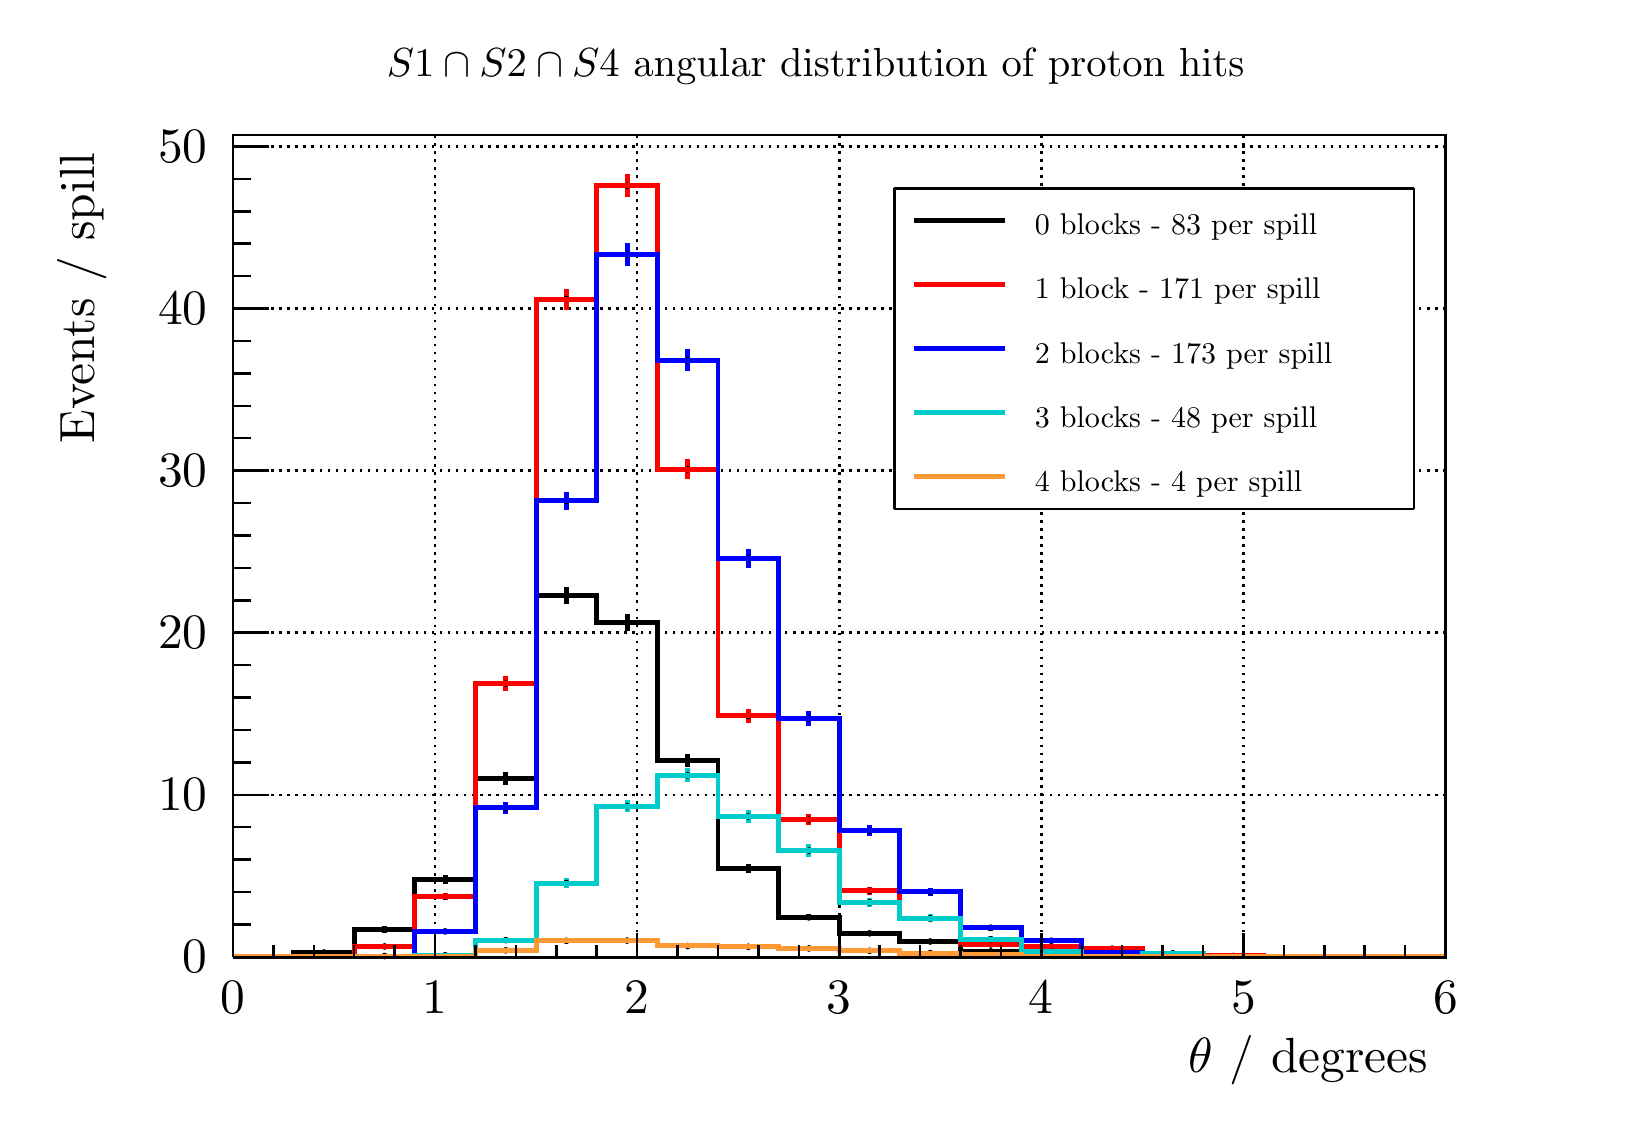
\begin{tikzpicture}
\pgfdeclareplotmark{cross} {
\pgfpathmoveto{\pgfpoint{-0.3\pgfplotmarksize}{\pgfplotmarksize}}
\pgfpathlineto{\pgfpoint{+0.3\pgfplotmarksize}{\pgfplotmarksize}}
\pgfpathlineto{\pgfpoint{+0.3\pgfplotmarksize}{0.3\pgfplotmarksize}}
\pgfpathlineto{\pgfpoint{+1\pgfplotmarksize}{0.3\pgfplotmarksize}}
\pgfpathlineto{\pgfpoint{+1\pgfplotmarksize}{-0.3\pgfplotmarksize}}
\pgfpathlineto{\pgfpoint{+0.3\pgfplotmarksize}{-0.3\pgfplotmarksize}}
\pgfpathlineto{\pgfpoint{+0.3\pgfplotmarksize}{-1.\pgfplotmarksize}}
\pgfpathlineto{\pgfpoint{-0.3\pgfplotmarksize}{-1.\pgfplotmarksize}}
\pgfpathlineto{\pgfpoint{-0.3\pgfplotmarksize}{-0.3\pgfplotmarksize}}
\pgfpathlineto{\pgfpoint{-1.\pgfplotmarksize}{-0.3\pgfplotmarksize}}
\pgfpathlineto{\pgfpoint{-1.\pgfplotmarksize}{0.3\pgfplotmarksize}}
\pgfpathlineto{\pgfpoint{-0.3\pgfplotmarksize}{0.3\pgfplotmarksize}}
\pgfpathclose
\pgfusepathqstroke
}
\pgfdeclareplotmark{cross*} {
\pgfpathmoveto{\pgfpoint{-0.3\pgfplotmarksize}{\pgfplotmarksize}}
\pgfpathlineto{\pgfpoint{+0.3\pgfplotmarksize}{\pgfplotmarksize}}
\pgfpathlineto{\pgfpoint{+0.3\pgfplotmarksize}{0.3\pgfplotmarksize}}
\pgfpathlineto{\pgfpoint{+1\pgfplotmarksize}{0.3\pgfplotmarksize}}
\pgfpathlineto{\pgfpoint{+1\pgfplotmarksize}{-0.3\pgfplotmarksize}}
\pgfpathlineto{\pgfpoint{+0.3\pgfplotmarksize}{-0.3\pgfplotmarksize}}
\pgfpathlineto{\pgfpoint{+0.3\pgfplotmarksize}{-1.\pgfplotmarksize}}
\pgfpathlineto{\pgfpoint{-0.3\pgfplotmarksize}{-1.\pgfplotmarksize}}
\pgfpathlineto{\pgfpoint{-0.3\pgfplotmarksize}{-0.3\pgfplotmarksize}}
\pgfpathlineto{\pgfpoint{-1.\pgfplotmarksize}{-0.3\pgfplotmarksize}}
\pgfpathlineto{\pgfpoint{-1.\pgfplotmarksize}{0.3\pgfplotmarksize}}
\pgfpathlineto{\pgfpoint{-0.3\pgfplotmarksize}{0.3\pgfplotmarksize}}
\pgfpathclose
\pgfusepathqfillstroke
}
\pgfdeclareplotmark{newstar} {
\pgfpathmoveto{\pgfqpoint{0pt}{\pgfplotmarksize}}
\pgfpathlineto{\pgfqpointpolar{44}{0.5\pgfplotmarksize}}
\pgfpathlineto{\pgfqpointpolar{18}{\pgfplotmarksize}}
\pgfpathlineto{\pgfqpointpolar{-20}{0.5\pgfplotmarksize}}
\pgfpathlineto{\pgfqpointpolar{-54}{\pgfplotmarksize}}
\pgfpathlineto{\pgfqpointpolar{-90}{0.5\pgfplotmarksize}}
\pgfpathlineto{\pgfqpointpolar{234}{\pgfplotmarksize}}
\pgfpathlineto{\pgfqpointpolar{198}{0.5\pgfplotmarksize}}
\pgfpathlineto{\pgfqpointpolar{162}{\pgfplotmarksize}}
\pgfpathlineto{\pgfqpointpolar{134}{0.5\pgfplotmarksize}}
\pgfpathclose
\pgfusepathqstroke
}
\pgfdeclareplotmark{newstar*} {
\pgfpathmoveto{\pgfqpoint{0pt}{\pgfplotmarksize}}
\pgfpathlineto{\pgfqpointpolar{44}{0.5\pgfplotmarksize}}
\pgfpathlineto{\pgfqpointpolar{18}{\pgfplotmarksize}}
\pgfpathlineto{\pgfqpointpolar{-20}{0.5\pgfplotmarksize}}
\pgfpathlineto{\pgfqpointpolar{-54}{\pgfplotmarksize}}
\pgfpathlineto{\pgfqpointpolar{-90}{0.5\pgfplotmarksize}}
\pgfpathlineto{\pgfqpointpolar{234}{\pgfplotmarksize}}
\pgfpathlineto{\pgfqpointpolar{198}{0.5\pgfplotmarksize}}
\pgfpathlineto{\pgfqpointpolar{162}{\pgfplotmarksize}}
\pgfpathlineto{\pgfqpointpolar{134}{0.5\pgfplotmarksize}}
\pgfpathclose
\pgfusepathqfillstroke
}
\definecolor{c}{rgb}{1,1,1};
\draw [color=c, fill=c] (0,0) rectangle (20,13.5632);
\draw [color=c, fill=c] (2.6,1.76322) rectangle (18,12.2069);
\definecolor{c}{rgb}{0,0,0};
\draw [c,line width=0.9] (2.6,1.76322) -- (2.6,12.2069) -- (18,12.2069) -- (18,1.76322) -- (2.6,1.76322);
\definecolor{c}{rgb}{1,1,1};
\draw [color=c, fill=c] (2.6,1.76322) rectangle (18,12.2069);
\definecolor{c}{rgb}{0,0,0};
\draw [c,line width=0.9] (2.6,1.76322) -- (2.6,12.2069) -- (18,12.2069) -- (18,1.76322) -- (2.6,1.76322);
\draw [c,line width=0.9] (2.6,1.76322) -- (18,1.76322);
\draw [c,dotted,line width=0.9] (2.6,12.2069) -- (2.6,1.76322);
\draw [c,dotted,line width=0.9] (5.16667,12.2069) -- (5.16667,1.76322);
\draw [c,dotted,line width=0.9] (7.73333,12.2069) -- (7.73333,1.76322);
\draw [c,dotted,line width=0.9] (10.3,12.2069) -- (10.3,1.76322);
\draw [c,dotted,line width=0.9] (12.8667,12.2069) -- (12.8667,1.76322);
\draw [c,dotted,line width=0.9] (15.4333,12.2069) -- (15.4333,1.76322);
\draw [c,dotted,line width=0.9] (18,12.2069) -- (18,1.76322);
\draw [c,line width=0.9] (2.6,1.76322) -- (2.6,12.2069);
\draw [c,dotted,line width=0.9] (18,1.76974) -- (2.6,1.76974);
\draw [c,dotted,line width=0.9] (18,3.82799) -- (2.6,3.82799);
\draw [c,dotted,line width=0.9] (18,5.88624) -- (2.6,5.88624);
\draw [c,dotted,line width=0.9] (18,7.94448) -- (2.6,7.94448);
\draw [c,dotted,line width=0.9] (18,10.0027) -- (2.6,10.0027);
\draw [c,dotted,line width=0.9] (18,12.061) -- (2.6,12.061);
\draw [c,dotted,line width=0.9] (18,1.76974) -- (2.6,1.76974);
\draw [c,dotted,line width=0.9] (18,12.061) -- (2.6,12.061);
\definecolor{c}{rgb}{0,0,0.6};
\draw [c,line width=0.9] (2.6,1.76974) -- (3.37,1.76974) -- (3.37,1.76974) -- (4.14,1.76974) -- (4.14,1.76974) -- (4.91,1.76974) -- (4.91,1.76974) -- (5.68,1.76974) -- (5.68,1.76974) -- (6.45,1.76974) -- (6.45,1.76974) -- (7.22,1.76974) --
 (7.22,1.76974) -- (7.99,1.76974) -- (7.99,1.76974) -- (8.76,1.76974) -- (8.76,1.76974) -- (9.53,1.76974) -- (9.53,1.76974) -- (10.3,1.76974) -- (10.3,1.76974) -- (11.07,1.76974) -- (11.07,1.76974) -- (11.84,1.76974) -- (11.84,1.76974) --
 (12.61,1.76974) -- (12.61,1.76974) -- (13.38,1.76974) -- (13.38,1.76974) -- (14.15,1.76974) -- (14.15,1.76974) -- (14.92,1.76974) -- (14.92,1.76974) -- (15.69,1.76974) -- (15.69,1.76974) -- (16.46,1.76974) -- (16.46,1.76974) -- (17.23,1.76974) --
 (17.23,1.76974) -- (18,1.76974);
\definecolor{c}{rgb}{0,0,0};
\draw [c,line width=0.9] (2.6,1.76322) -- (18,1.76322);
\draw [anchor= east] (18,0.461149) node[scale=1.78699, color=c, rotate=0]{$\theta$ / degrees};
\draw [c,line width=0.9] (2.6,2.07653) -- (2.6,1.76322);
\draw [c,line width=0.9] (3.11333,1.91987) -- (3.11333,1.76322);
\draw [c,line width=0.9] (3.62667,1.91987) -- (3.62667,1.76322);
\draw [c,line width=0.9] (4.14,1.91987) -- (4.14,1.76322);
\draw [c,line width=0.9] (4.65333,1.91987) -- (4.65333,1.76322);
\draw [c,line width=0.9] (5.16667,2.07653) -- (5.16667,1.76322);
\draw [c,line width=0.9] (5.68,1.91987) -- (5.68,1.76322);
\draw [c,line width=0.9] (6.19333,1.91987) -- (6.19333,1.76322);
\draw [c,line width=0.9] (6.70667,1.91987) -- (6.70667,1.76322);
\draw [c,line width=0.9] (7.22,1.91987) -- (7.22,1.76322);
\draw [c,line width=0.9] (7.73333,2.07653) -- (7.73333,1.76322);
\draw [c,line width=0.9] (8.24667,1.91987) -- (8.24667,1.76322);
\draw [c,line width=0.9] (8.76,1.91987) -- (8.76,1.76322);
\draw [c,line width=0.9] (9.27333,1.91987) -- (9.27333,1.76322);
\draw [c,line width=0.9] (9.78667,1.91987) -- (9.78667,1.76322);
\draw [c,line width=0.9] (10.3,2.07653) -- (10.3,1.76322);
\draw [c,line width=0.9] (10.8133,1.91987) -- (10.8133,1.76322);
\draw [c,line width=0.9] (11.3267,1.91987) -- (11.3267,1.76322);
\draw [c,line width=0.9] (11.84,1.91987) -- (11.84,1.76322);
\draw [c,line width=0.9] (12.3533,1.91987) -- (12.3533,1.76322);
\draw [c,line width=0.9] (12.8667,2.07653) -- (12.8667,1.76322);
\draw [c,line width=0.9] (13.38,1.91987) -- (13.38,1.76322);
\draw [c,line width=0.9] (13.8933,1.91987) -- (13.8933,1.76322);
\draw [c,line width=0.9] (14.4067,1.91987) -- (14.4067,1.76322);
\draw [c,line width=0.9] (14.92,1.91987) -- (14.92,1.76322);
\draw [c,line width=0.9] (15.4333,2.07653) -- (15.4333,1.76322);
\draw [c,line width=0.9] (15.9467,1.91987) -- (15.9467,1.76322);
\draw [c,line width=0.9] (16.46,1.91987) -- (16.46,1.76322);
\draw [c,line width=0.9] (16.9733,1.91987) -- (16.9733,1.76322);
\draw [c,line width=0.9] (17.4867,1.91987) -- (17.4867,1.76322);
\draw [c,line width=0.9] (18,2.07653) -- (18,1.76322);
\draw [anchor=base] (2.6,1.04437) node[scale=1.78699, color=c, rotate=0]{0};
\draw [anchor=base] (5.16667,1.04437) node[scale=1.78699, color=c, rotate=0]{1};
\draw [anchor=base] (7.73333,1.04437) node[scale=1.78699, color=c, rotate=0]{2};
\draw [anchor=base] (10.3,1.04437) node[scale=1.78699, color=c, rotate=0]{3};
\draw [anchor=base] (12.8667,1.04437) node[scale=1.78699, color=c, rotate=0]{4};
\draw [anchor=base] (15.4333,1.04437) node[scale=1.78699, color=c, rotate=0]{5};
\draw [anchor=base] (18,1.04437) node[scale=1.78699, color=c, rotate=0]{6};
\draw [c,line width=0.9] (2.6,1.76322) -- (2.6,12.2069);
\draw [anchor= east] (0.68,12.2069) node[scale=1.78699, color=c, rotate=90]{ Events / spill};
\draw [c,line width=0.9] (3.062,1.76974) -- (2.6,1.76974);
\draw [c,line width=0.9] (2.831,2.18139) -- (2.6,2.18139);
\draw [c,line width=0.9] (2.831,2.59304) -- (2.6,2.59304);
\draw [c,line width=0.9] (2.831,3.00469) -- (2.6,3.00469);
\draw [c,line width=0.9] (2.831,3.41634) -- (2.6,3.41634);
\draw [c,line width=0.9] (3.062,3.82799) -- (2.6,3.82799);
\draw [c,line width=0.9] (2.831,4.23964) -- (2.6,4.23964);
\draw [c,line width=0.9] (2.831,4.65129) -- (2.6,4.65129);
\draw [c,line width=0.9] (2.831,5.06294) -- (2.6,5.06294);
\draw [c,line width=0.9] (2.831,5.47459) -- (2.6,5.47459);
\draw [c,line width=0.9] (3.062,5.88624) -- (2.6,5.88624);
\draw [c,line width=0.9] (2.831,6.29789) -- (2.6,6.29789);
\draw [c,line width=0.9] (2.831,6.70953) -- (2.6,6.70953);
\draw [c,line width=0.9] (2.831,7.12118) -- (2.6,7.12118);
\draw [c,line width=0.9] (2.831,7.53283) -- (2.6,7.53283);
\draw [c,line width=0.9] (3.062,7.94448) -- (2.6,7.94448);
\draw [c,line width=0.9] (2.831,8.35613) -- (2.6,8.35613);
\draw [c,line width=0.9] (2.831,8.76778) -- (2.6,8.76778);
\draw [c,line width=0.9] (2.831,9.17943) -- (2.6,9.17943);
\draw [c,line width=0.9] (2.831,9.59108) -- (2.6,9.59108);
\draw [c,line width=0.9] (3.062,10.0027) -- (2.6,10.0027);
\draw [c,line width=0.9] (2.831,10.4144) -- (2.6,10.4144);
\draw [c,line width=0.9] (2.831,10.826) -- (2.6,10.826);
\draw [c,line width=0.9] (2.831,11.2377) -- (2.6,11.2377);
\draw [c,line width=0.9] (2.831,11.6493) -- (2.6,11.6493);
\draw [c,line width=0.9] (3.062,12.061) -- (2.6,12.061);
\draw [c,line width=0.9] (3.062,1.76974) -- (2.6,1.76974);
\draw [c,line width=0.9] (3.062,12.061) -- (2.6,12.061);
\draw [anchor= east] (2.5,1.76974) node[scale=1.78699, color=c, rotate=0]{0};
\draw [anchor= east] (2.5,3.82799) node[scale=1.78699, color=c, rotate=0]{10};
\draw [anchor= east] (2.5,5.88624) node[scale=1.78699, color=c, rotate=0]{20};
\draw [anchor= east] (2.5,7.94448) node[scale=1.78699, color=c, rotate=0]{30};
\draw [anchor= east] (2.5,10.0027) node[scale=1.78699, color=c, rotate=0]{40};
\draw [anchor= east] (2.5,12.061) node[scale=1.78699, color=c, rotate=0]{50};
\draw [c,line width=1.8] (3.755,1.80661) -- (3.755,1.82512);
\draw [c,line width=1.8] (3.755,1.82512) -- (3.755,1.84364);
\foreach \P in {(3.755,1.82512)}{\draw[mark options={color=c,fill=c},mark size=2.402402pt,mark=*,mark size=1pt] plot coordinates {\P};}
\draw [c,line width=1.8] (4.525,2.07739) -- (4.525,2.11837);
\draw [c,line width=1.8] (4.525,2.11837) -- (4.525,2.15935);
\foreach \P in {(4.525,2.11837)}{\draw[mark options={color=c,fill=c},mark size=2.402402pt,mark=*,mark size=1pt] plot coordinates {\P};}
\draw [c,line width=1.8] (5.295,2.68979) -- (5.295,2.75208);
\draw [c,line width=1.8] (5.295,2.75208) -- (5.295,2.81437);
\foreach \P in {(5.295,2.75208)}{\draw[mark options={color=c,fill=c},mark size=2.402402pt,mark=*,mark size=1pt] plot coordinates {\P};}
\draw [c,line width=1.8] (6.065,3.94712) -- (6.065,4.03136);
\draw [c,line width=1.8] (6.065,4.03136) -- (6.065,4.11561);
\foreach \P in {(6.065,4.03136)}{\draw[mark options={color=c,fill=c},mark size=2.402402pt,mark=*,mark size=1pt] plot coordinates {\P};}
\draw [c,line width=1.8] (6.835,6.25543) -- (6.835,6.36302);
\draw [c,line width=1.8] (6.835,6.36302) -- (6.835,6.4706);
\foreach \P in {(6.835,6.36302)}{\draw[mark options={color=c,fill=c},mark size=2.402402pt,mark=*,mark size=1pt] plot coordinates {\P};}
\draw [c,line width=1.8] (7.605,5.91374) -- (7.605,6.01656);
\draw [c,line width=1.8] (7.605,6.01656) -- (7.605,6.11939);
\foreach \P in {(7.605,6.01656)}{\draw[mark options={color=c,fill=c},mark size=2.402402pt,mark=*,mark size=1pt] plot coordinates {\P};}
\draw [c,line width=1.8] (8.375,4.18387) -- (8.375,4.26602);
\draw [c,line width=1.8] (8.375,4.26602) -- (8.375,4.34818);
\foreach \P in {(8.375,4.26602)}{\draw[mark options={color=c,fill=c},mark size=2.402402pt,mark=*,mark size=1pt] plot coordinates {\P};}
\draw [c,line width=1.8] (9.145,2.83028) -- (9.145,2.8869);
\draw [c,line width=1.8] (9.145,2.8869) -- (9.145,2.94353);
\foreach \P in {(9.145,2.8869)}{\draw[mark options={color=c,fill=c},mark size=2.402402pt,mark=*,mark size=1pt] plot coordinates {\P};}
\draw [c,line width=1.8] (9.915,2.2324) -- (9.915,2.27092);
\draw [c,line width=1.8] (9.915,2.27092) -- (9.915,2.30944);
\foreach \P in {(9.915,2.27092)}{\draw[mark options={color=c,fill=c},mark size=2.402402pt,mark=*,mark size=1pt] plot coordinates {\P};}
\draw [c,line width=1.8] (10.685,2.03761) -- (10.685,2.06803);
\draw [c,line width=1.8] (10.685,2.06803) -- (10.685,2.09845);
\foreach \P in {(10.685,2.06803)}{\draw[mark options={color=c,fill=c},mark size=2.402402pt,mark=*,mark size=1pt] plot coordinates {\P};}
\draw [c,line width=1.8] (11.455,1.94017) -- (11.455,1.96434);
\draw [c,line width=1.8] (11.455,1.96434) -- (11.455,1.98852);
\foreach \P in {(11.455,1.96434)}{\draw[mark options={color=c,fill=c},mark size=2.402402pt,mark=*,mark size=1pt] plot coordinates {\P};}
\draw [c,line width=1.8] (12.225,1.82355) -- (12.225,1.83903);
\draw [c,line width=1.8] (12.225,1.83903) -- (12.225,1.85452);
\foreach \P in {(12.225,1.83903)}{\draw[mark options={color=c,fill=c},mark size=2.402402pt,mark=*,mark size=1pt] plot coordinates {\P};}
\draw [c,line width=1.8] (12.995,1.80676) -- (12.995,1.82057);
\draw [c,line width=1.8] (12.995,1.82057) -- (12.995,1.83438);
\foreach \P in {(12.995,1.82057)}{\draw[mark options={color=c,fill=c},mark size=2.402402pt,mark=*,mark size=1pt] plot coordinates {\P};}
\draw [c,line width=1.8] (13.765,1.77723) -- (13.765,1.78745);
\draw [c,line width=1.8] (13.765,1.78745) -- (13.765,1.79768);
\foreach \P in {(13.765,1.78745)}{\draw[mark options={color=c,fill=c},mark size=2.402402pt,mark=*,mark size=1pt] plot coordinates {\P};}
\draw [c,line width=1.8] (14.535,1.78362) -- (14.535,1.79604);
\draw [c,line width=1.8] (14.535,1.79604) -- (14.535,1.80845);
\foreach \P in {(14.535,1.79604)}{\draw[mark options={color=c,fill=c},mark size=2.402402pt,mark=*,mark size=1pt] plot coordinates {\P};}
\draw [c,line width=1.8] (2.6,1.76974) -- (3.37,1.76974) -- (3.37,1.82512) -- (4.14,1.82512) -- (4.14,2.11837) -- (4.91,2.11837) -- (4.91,2.75208) -- (5.68,2.75208) -- (5.68,4.03136) -- (6.45,4.03136) -- (6.45,6.36302) -- (7.22,6.36302) --
 (7.22,6.01656) -- (7.99,6.01656) -- (7.99,4.26602) -- (8.76,4.26602) -- (8.76,2.8869) -- (9.53,2.8869) -- (9.53,2.27092) -- (10.3,2.27092) -- (10.3,2.06803) -- (11.07,2.06803) -- (11.07,1.96434) -- (11.84,1.96434) -- (11.84,1.83903) --
 (12.61,1.83903) -- (12.61,1.82057) -- (13.38,1.82057) -- (13.38,1.78745) -- (14.15,1.78745) -- (14.15,1.79604) -- (14.92,1.79604) -- (14.92,1.76974) -- (15.69,1.76974) -- (15.69,1.76974) -- (16.46,1.76974) -- (16.46,1.76974) -- (17.23,1.76974) --
 (17.23,1.76974) -- (18,1.76974);
\definecolor{c}{rgb}{1,0,0};
\draw [c,line width=1.8] (4.525,1.87963) -- (4.525,1.90177);
\draw [c,line width=1.8] (4.525,1.90177) -- (4.525,1.92392);
\definecolor{c}{rgb}{0,0,0};
\foreach \P in {(4.525,1.90177)}{\draw[mark options={color=c,fill=c},mark size=2.402402pt,mark=*,mark size=1pt] plot coordinates {\P};}
\definecolor{c}{rgb}{1,0,0};
\draw [c,line width=1.8] (5.295,2.48842) -- (5.295,2.53379);
\draw [c,line width=1.8] (5.295,2.53379) -- (5.295,2.57917);
\definecolor{c}{rgb}{0,0,0};
\foreach \P in {(5.295,2.53379)}{\draw[mark options={color=c,fill=c},mark size=2.402402pt,mark=*,mark size=1pt] plot coordinates {\P};}
\definecolor{c}{rgb}{1,0,0};
\draw [c,line width=1.8] (6.065,5.14757) -- (6.065,5.23916);
\draw [c,line width=1.8] (6.065,5.23916) -- (6.065,5.33075);
\definecolor{c}{rgb}{0,0,0};
\foreach \P in {(6.065,5.23916)}{\draw[mark options={color=c,fill=c},mark size=2.402402pt,mark=*,mark size=1pt] plot coordinates {\P};}
\definecolor{c}{rgb}{1,0,0};
\draw [c,line width=1.8] (6.835,9.98824) -- (6.835,10.1229);
\draw [c,line width=1.8] (6.835,10.1229) -- (6.835,10.2575);
\definecolor{c}{rgb}{0,0,0};
\foreach \P in {(6.835,10.1229)}{\draw[mark options={color=c,fill=c},mark size=2.402402pt,mark=*,mark size=1pt] plot coordinates {\P};}
\definecolor{c}{rgb}{1,0,0};
\draw [c,line width=1.8] (7.605,11.4135) -- (7.605,11.5617);
\draw [c,line width=1.8] (7.605,11.5617) -- (7.605,11.7099);
\definecolor{c}{rgb}{0,0,0};
\foreach \P in {(7.605,11.5617)}{\draw[mark options={color=c,fill=c},mark size=2.402402pt,mark=*,mark size=1pt] plot coordinates {\P};}
\definecolor{c}{rgb}{1,0,0};
\draw [c,line width=1.8] (8.375,7.83438) -- (8.375,7.96218);
\draw [c,line width=1.8] (8.375,7.96218) -- (8.375,8.08997);
\definecolor{c}{rgb}{0,0,0};
\foreach \P in {(8.375,7.96218)}{\draw[mark options={color=c,fill=c},mark size=2.402402pt,mark=*,mark size=1pt] plot coordinates {\P};}
\definecolor{c}{rgb}{1,0,0};
\draw [c,line width=1.8] (9.145,4.7362) -- (9.145,4.8288);
\draw [c,line width=1.8] (9.145,4.8288) -- (9.145,4.92141);
\definecolor{c}{rgb}{0,0,0};
\foreach \P in {(9.145,4.8288)}{\draw[mark options={color=c,fill=c},mark size=2.402402pt,mark=*,mark size=1pt] plot coordinates {\P};}
\definecolor{c}{rgb}{1,0,0};
\draw [c,line width=1.8] (9.915,3.44189) -- (9.915,3.51287);
\draw [c,line width=1.8] (9.915,3.51287) -- (9.915,3.58386);
\definecolor{c}{rgb}{0,0,0};
\foreach \P in {(9.915,3.51287)}{\draw[mark options={color=c,fill=c},mark size=2.402402pt,mark=*,mark size=1pt] plot coordinates {\P};}
\definecolor{c}{rgb}{1,0,0};
\draw [c,line width=1.8] (10.685,2.55853) -- (10.685,2.60881);
\draw [c,line width=1.8] (10.685,2.60881) -- (10.685,2.65908);
\definecolor{c}{rgb}{0,0,0};
\foreach \P in {(10.685,2.60881)}{\draw[mark options={color=c,fill=c},mark size=2.402402pt,mark=*,mark size=1pt] plot coordinates {\P};}
\definecolor{c}{rgb}{1,0,0};
\draw [c,line width=1.8] (11.455,2.21208) -- (11.455,2.25177);
\draw [c,line width=1.8] (11.455,2.25177) -- (11.455,2.29147);
\definecolor{c}{rgb}{0,0,0};
\foreach \P in {(11.455,2.25177)}{\draw[mark options={color=c,fill=c},mark size=2.402402pt,mark=*,mark size=1pt] plot coordinates {\P};}
\definecolor{c}{rgb}{1,0,0};
\draw [c,line width=1.8] (12.225,1.90513) -- (12.225,1.92751);
\draw [c,line width=1.8] (12.225,1.92751) -- (12.225,1.94988);
\definecolor{c}{rgb}{0,0,0};
\foreach \P in {(12.225,1.92751)}{\draw[mark options={color=c,fill=c},mark size=2.402402pt,mark=*,mark size=1pt] plot coordinates {\P};}
\definecolor{c}{rgb}{1,0,0};
\draw [c,line width=1.8] (12.995,1.87998) -- (12.995,1.90117);
\draw [c,line width=1.8] (12.995,1.90117) -- (12.995,1.92236);
\definecolor{c}{rgb}{0,0,0};
\foreach \P in {(12.995,1.90117)}{\draw[mark options={color=c,fill=c},mark size=2.402402pt,mark=*,mark size=1pt] plot coordinates {\P};}
\definecolor{c}{rgb}{1,0,0};
\draw [c,line width=1.8] (13.765,1.85362) -- (13.765,1.87401);
\draw [c,line width=1.8] (13.765,1.87401) -- (13.765,1.8944);
\definecolor{c}{rgb}{0,0,0};
\foreach \P in {(13.765,1.87401)}{\draw[mark options={color=c,fill=c},mark size=2.402402pt,mark=*,mark size=1pt] plot coordinates {\P};}
\definecolor{c}{rgb}{1,0,0};
\draw [c,line width=1.8] (14.535,1.78966) -- (14.535,1.80321);
\draw [c,line width=1.8] (14.535,1.80321) -- (14.535,1.81677);
\definecolor{c}{rgb}{0,0,0};
\foreach \P in {(14.535,1.80321)}{\draw[mark options={color=c,fill=c},mark size=2.402402pt,mark=*,mark size=1pt] plot coordinates {\P};}
\definecolor{c}{rgb}{1,0,0};
\draw [c,line width=1.8] (15.305,1.76743) -- (15.305,1.78116);
\draw [c,line width=1.8] (15.305,1.78116) -- (15.305,1.79489);
\definecolor{c}{rgb}{0,0,0};
\foreach \P in {(15.305,1.78116)}{\draw[mark options={color=c,fill=c},mark size=2.402402pt,mark=*,mark size=1pt] plot coordinates {\P};}
\definecolor{c}{rgb}{1,0,0};
\draw [c,line width=1.8] (2.6,1.76974) -- (3.37,1.76974) -- (3.37,1.76974) -- (4.14,1.76974) -- (4.14,1.90177) -- (4.91,1.90177) -- (4.91,2.53379) -- (5.68,2.53379) -- (5.68,5.23916) -- (6.45,5.23916) -- (6.45,10.1229) -- (7.22,10.1229) --
 (7.22,11.5617) -- (7.99,11.5617) -- (7.99,7.96218) -- (8.76,7.96218) -- (8.76,4.8288) -- (9.53,4.8288) -- (9.53,3.51287) -- (10.3,3.51287) -- (10.3,2.60881) -- (11.07,2.60881) -- (11.07,2.25177) -- (11.84,2.25177) -- (11.84,1.92751) --
 (12.61,1.92751) -- (12.61,1.90117) -- (13.38,1.90117) -- (13.38,1.87401) -- (14.15,1.87401) -- (14.15,1.80321) -- (14.92,1.80321) -- (14.92,1.78116) -- (15.69,1.78116) -- (15.69,1.76974) -- (16.46,1.76974) -- (16.46,1.76974) -- (17.23,1.76974) --
 (17.23,1.76974) -- (18,1.76974);
\definecolor{c}{rgb}{0,0,1};
\draw [c,line width=1.8] (4.525,1.76322) -- (4.525,1.77991);
\draw [c,line width=1.8] (4.525,1.77991) -- (4.525,1.7966);
\definecolor{c}{rgb}{0,0,0};
\foreach \P in {(4.525,1.77991)}{\draw[mark options={color=c,fill=c},mark size=2.402402pt,mark=*,mark size=1pt] plot coordinates {\P};}
\definecolor{c}{rgb}{0,0,1};
\draw [c,line width=1.8] (5.295,2.05961) -- (5.295,2.09263);
\draw [c,line width=1.8] (5.295,2.09263) -- (5.295,2.12565);
\definecolor{c}{rgb}{0,0,0};
\foreach \P in {(5.295,2.09263)}{\draw[mark options={color=c,fill=c},mark size=2.402402pt,mark=*,mark size=1pt] plot coordinates {\P};}
\definecolor{c}{rgb}{0,0,1};
\draw [c,line width=1.8] (6.065,3.58922) -- (6.065,3.66036);
\draw [c,line width=1.8] (6.065,3.66036) -- (6.065,3.7315);
\definecolor{c}{rgb}{0,0,0};
\foreach \P in {(6.065,3.66036)}{\draw[mark options={color=c,fill=c},mark size=2.402402pt,mark=*,mark size=1pt] plot coordinates {\P};}
\definecolor{c}{rgb}{0,0,1};
\draw [c,line width=1.8] (6.835,7.44282) -- (6.835,7.56041);
\draw [c,line width=1.8] (6.835,7.56041) -- (6.835,7.678);
\definecolor{c}{rgb}{0,0,0};
\foreach \P in {(6.835,7.56041)}{\draw[mark options={color=c,fill=c},mark size=2.402402pt,mark=*,mark size=1pt] plot coordinates {\P};}
\definecolor{c}{rgb}{0,0,1};
\draw [c,line width=1.8] (7.605,10.5479) -- (7.605,10.6894);
\draw [c,line width=1.8] (7.605,10.6894) -- (7.605,10.8309);
\definecolor{c}{rgb}{0,0,0};
\foreach \P in {(7.605,10.6894)}{\draw[mark options={color=c,fill=c},mark size=2.402402pt,mark=*,mark size=1pt] plot coordinates {\P};}
\definecolor{c}{rgb}{0,0,1};
\draw [c,line width=1.8] (8.375,9.20775) -- (8.375,9.34629);
\draw [c,line width=1.8] (8.375,9.34629) -- (8.375,9.48483);
\definecolor{c}{rgb}{0,0,0};
\foreach \P in {(8.375,9.34629)}{\draw[mark options={color=c,fill=c},mark size=2.402402pt,mark=*,mark size=1pt] plot coordinates {\P};}
\definecolor{c}{rgb}{0,0,1};
\draw [c,line width=1.8] (9.145,6.70824) -- (9.145,6.83094);
\draw [c,line width=1.8] (9.145,6.83094) -- (9.145,6.95365);
\definecolor{c}{rgb}{0,0,0};
\foreach \P in {(9.145,6.83094)}{\draw[mark options={color=c,fill=c},mark size=2.402402pt,mark=*,mark size=1pt] plot coordinates {\P};}
\definecolor{c}{rgb}{0,0,1};
\draw [c,line width=1.8] (9.915,4.7009) -- (9.915,4.79746);
\draw [c,line width=1.8] (9.915,4.79746) -- (9.915,4.89402);
\definecolor{c}{rgb}{0,0,0};
\foreach \P in {(9.915,4.79746)}{\draw[mark options={color=c,fill=c},mark size=2.402402pt,mark=*,mark size=1pt] plot coordinates {\P};}
\definecolor{c}{rgb}{0,0,1};
\draw [c,line width=1.8] (10.685,3.30018) -- (10.685,3.36965);
\draw [c,line width=1.8] (10.685,3.36965) -- (10.685,3.43912);
\definecolor{c}{rgb}{0,0,0};
\foreach \P in {(10.685,3.36965)}{\draw[mark options={color=c,fill=c},mark size=2.402402pt,mark=*,mark size=1pt] plot coordinates {\P};}
\definecolor{c}{rgb}{0,0,1};
\draw [c,line width=1.8] (11.455,2.54232) -- (11.455,2.59381);
\draw [c,line width=1.8] (11.455,2.59381) -- (11.455,2.64531);
\definecolor{c}{rgb}{0,0,0};
\foreach \P in {(11.455,2.59381)}{\draw[mark options={color=c,fill=c},mark size=2.402402pt,mark=*,mark size=1pt] plot coordinates {\P};}
\definecolor{c}{rgb}{0,0,1};
\draw [c,line width=1.8] (12.225,2.10415) -- (12.225,2.13998);
\draw [c,line width=1.8] (12.225,2.13998) -- (12.225,2.1758);
\definecolor{c}{rgb}{0,0,0};
\foreach \P in {(12.225,2.13998)}{\draw[mark options={color=c,fill=c},mark size=2.402402pt,mark=*,mark size=1pt] plot coordinates {\P};}
\definecolor{c}{rgb}{0,0,1};
\draw [c,line width=1.8] (12.995,1.94759) -- (12.995,1.9747);
\draw [c,line width=1.8] (12.995,1.9747) -- (12.995,2.00181);
\definecolor{c}{rgb}{0,0,0};
\foreach \P in {(12.995,1.9747)}{\draw[mark options={color=c,fill=c},mark size=2.402402pt,mark=*,mark size=1pt] plot coordinates {\P};}
\definecolor{c}{rgb}{0,0,1};
\draw [c,line width=1.8] (13.765,1.8042) -- (13.765,1.82296);
\draw [c,line width=1.8] (13.765,1.82296) -- (13.765,1.84173);
\definecolor{c}{rgb}{0,0,0};
\foreach \P in {(13.765,1.82296)}{\draw[mark options={color=c,fill=c},mark size=2.402402pt,mark=*,mark size=1pt] plot coordinates {\P};}
\definecolor{c}{rgb}{0,0,1};
\draw [c,line width=1.8] (14.535,1.79476) -- (14.535,1.8142);
\draw [c,line width=1.8] (14.535,1.8142) -- (14.535,1.83364);
\definecolor{c}{rgb}{0,0,0};
\foreach \P in {(14.535,1.8142)}{\draw[mark options={color=c,fill=c},mark size=2.402402pt,mark=*,mark size=1pt] plot coordinates {\P};}
\definecolor{c}{rgb}{0,0,1};
\draw [c,line width=1.8] (2.6,1.76974) -- (3.37,1.76974) -- (3.37,1.76974) -- (4.14,1.76974) -- (4.14,1.77991) -- (4.91,1.77991) -- (4.91,2.09263) -- (5.68,2.09263) -- (5.68,3.66036) -- (6.45,3.66036) -- (6.45,7.56041) -- (7.22,7.56041) --
 (7.22,10.6894) -- (7.99,10.6894) -- (7.99,9.34629) -- (8.76,9.34629) -- (8.76,6.83094) -- (9.53,6.83094) -- (9.53,4.79746) -- (10.3,4.79746) -- (10.3,3.36965) -- (11.07,3.36965) -- (11.07,2.59381) -- (11.84,2.59381) -- (11.84,2.13998) --
 (12.61,2.13998) -- (12.61,1.9747) -- (13.38,1.9747) -- (13.38,1.82296) -- (14.15,1.82296) -- (14.15,1.8142) -- (14.92,1.8142) -- (14.92,1.76974) -- (15.69,1.76974) -- (15.69,1.76974) -- (16.46,1.76974) -- (16.46,1.76974) -- (17.23,1.76974) --
 (17.23,1.76974) -- (18,1.76974);
\definecolor{c}{rgb}{0,0.8,0.8};
\draw [c,line width=1.8] (5.295,1.77228) -- (5.295,1.79003);
\draw [c,line width=1.8] (5.295,1.79003) -- (5.295,1.80777);
\definecolor{c}{rgb}{0,0,0};
\foreach \P in {(5.295,1.79003)}{\draw[mark options={color=c,fill=c},mark size=2.402402pt,mark=*,mark size=1pt] plot coordinates {\P};}
\definecolor{c}{rgb}{0,0.8,0.8};
\draw [c,line width=1.8] (6.065,1.95127) -- (6.065,1.98182);
\draw [c,line width=1.8] (6.065,1.98182) -- (6.065,2.01237);
\definecolor{c}{rgb}{0,0,0};
\foreach \P in {(6.065,1.98182)}{\draw[mark options={color=c,fill=c},mark size=2.402402pt,mark=*,mark size=1pt] plot coordinates {\P};}
\definecolor{c}{rgb}{0,0.8,0.8};
\draw [c,line width=1.8] (6.835,2.6487) -- (6.835,2.70736);
\draw [c,line width=1.8] (6.835,2.70736) -- (6.835,2.76602);
\definecolor{c}{rgb}{0,0,0};
\foreach \P in {(6.835,2.70736)}{\draw[mark options={color=c,fill=c},mark size=2.402402pt,mark=*,mark size=1pt] plot coordinates {\P};}
\definecolor{c}{rgb}{0,0.8,0.8};
\draw [c,line width=1.8] (7.605,3.60528) -- (7.605,3.68176);
\draw [c,line width=1.8] (7.605,3.68176) -- (7.605,3.75823);
\definecolor{c}{rgb}{0,0,0};
\foreach \P in {(7.605,3.68176)}{\draw[mark options={color=c,fill=c},mark size=2.402402pt,mark=*,mark size=1pt] plot coordinates {\P};}
\definecolor{c}{rgb}{0,0.8,0.8};
\draw [c,line width=1.8] (8.375,3.98782) -- (8.375,4.07498);
\draw [c,line width=1.8] (8.375,4.07498) -- (8.375,4.16215);
\definecolor{c}{rgb}{0,0,0};
\foreach \P in {(8.375,4.07498)}{\draw[mark options={color=c,fill=c},mark size=2.402402pt,mark=*,mark size=1pt] plot coordinates {\P};}
\definecolor{c}{rgb}{0,0.8,0.8};
\draw [c,line width=1.8] (9.145,3.46512) -- (9.145,3.55291);
\draw [c,line width=1.8] (9.145,3.55291) -- (9.145,3.64071);
\definecolor{c}{rgb}{0,0,0};
\foreach \P in {(9.145,3.55291)}{\draw[mark options={color=c,fill=c},mark size=2.402402pt,mark=*,mark size=1pt] plot coordinates {\P};}
\definecolor{c}{rgb}{0,0.8,0.8};
\draw [c,line width=1.8] (9.915,3.03822) -- (9.915,3.11967);
\draw [c,line width=1.8] (9.915,3.11967) -- (9.915,3.20111);
\definecolor{c}{rgb}{0,0,0};
\foreach \P in {(9.915,3.11967)}{\draw[mark options={color=c,fill=c},mark size=2.402402pt,mark=*,mark size=1pt] plot coordinates {\P};}
\definecolor{c}{rgb}{0,0.8,0.8};
\draw [c,line width=1.8] (10.685,2.40584) -- (10.685,2.46168);
\draw [c,line width=1.8] (10.685,2.46168) -- (10.685,2.51752);
\definecolor{c}{rgb}{0,0,0};
\foreach \P in {(10.685,2.46168)}{\draw[mark options={color=c,fill=c},mark size=2.402402pt,mark=*,mark size=1pt] plot coordinates {\P};}
\definecolor{c}{rgb}{0,0.8,0.8};
\draw [c,line width=1.8] (11.455,2.20959) -- (11.455,2.25887);
\draw [c,line width=1.8] (11.455,2.25887) -- (11.455,2.30816);
\definecolor{c}{rgb}{0,0,0};
\foreach \P in {(11.455,2.25887)}{\draw[mark options={color=c,fill=c},mark size=2.402402pt,mark=*,mark size=1pt] plot coordinates {\P};}
\definecolor{c}{rgb}{0,0.8,0.8};
\draw [c,line width=1.8] (12.225,1.95579) -- (12.225,1.99241);
\draw [c,line width=1.8] (12.225,1.99241) -- (12.225,2.02902);
\definecolor{c}{rgb}{0,0,0};
\foreach \P in {(12.225,1.99241)}{\draw[mark options={color=c,fill=c},mark size=2.402402pt,mark=*,mark size=1pt] plot coordinates {\P};}
\definecolor{c}{rgb}{0,0.8,0.8};
\draw [c,line width=1.8] (12.995,1.81125) -- (12.995,1.83513);
\draw [c,line width=1.8] (12.995,1.83513) -- (12.995,1.85902);
\definecolor{c}{rgb}{0,0,0};
\foreach \P in {(12.995,1.83513)}{\draw[mark options={color=c,fill=c},mark size=2.402402pt,mark=*,mark size=1pt] plot coordinates {\P};}
\definecolor{c}{rgb}{0,0.8,0.8};
\draw [c,line width=1.8] (14.535,1.78658) -- (14.535,1.80979);
\draw [c,line width=1.8] (14.535,1.80979) -- (14.535,1.83299);
\definecolor{c}{rgb}{0,0,0};
\foreach \P in {(14.535,1.80979)}{\draw[mark options={color=c,fill=c},mark size=2.402402pt,mark=*,mark size=1pt] plot coordinates {\P};}
\definecolor{c}{rgb}{0,0.8,0.8};
\draw [c,line width=1.8] (2.6,1.76974) -- (3.37,1.76974) -- (3.37,1.76974) -- (4.14,1.76974) -- (4.14,1.76974) -- (4.91,1.76974) -- (4.91,1.79003) -- (5.68,1.79003) -- (5.68,1.98182) -- (6.45,1.98182) -- (6.45,2.70736) -- (7.22,2.70736) --
 (7.22,3.68176) -- (7.99,3.68176) -- (7.99,4.07498) -- (8.76,4.07498) -- (8.76,3.55291) -- (9.53,3.55291) -- (9.53,3.11967) -- (10.3,3.11967) -- (10.3,2.46168) -- (11.07,2.46168) -- (11.07,2.25887) -- (11.84,2.25887) -- (11.84,1.99241) --
 (12.61,1.99241) -- (12.61,1.83513) -- (13.38,1.83513) -- (13.38,1.76974) -- (14.15,1.76974) -- (14.15,1.80979) -- (14.92,1.80979) -- (14.92,1.76974) -- (15.69,1.76974) -- (15.69,1.76974) -- (16.46,1.76974) -- (16.46,1.76974) -- (17.23,1.76974) --
 (17.23,1.76974) -- (18,1.76974);
\definecolor{c}{rgb}{1,0.6,0.2};
\draw [c,line width=1.8] (6.065,1.84606) -- (6.065,1.85249);
\draw [c,line width=1.8] (6.065,1.85249) -- (6.065,1.85892);
\definecolor{c}{rgb}{0,0,0};
\foreach \P in {(6.065,1.85249)}{\draw[mark options={color=c,fill=c},mark size=2.402402pt,mark=*,mark size=1pt] plot coordinates {\P};}
\definecolor{c}{rgb}{1,0.6,0.2};
\draw [c,line width=1.8] (6.835,1.96547) -- (6.835,1.97312);
\draw [c,line width=1.8] (6.835,1.97312) -- (6.835,1.98077);
\definecolor{c}{rgb}{0,0,0};
\foreach \P in {(6.835,1.97312)}{\draw[mark options={color=c,fill=c},mark size=2.402402pt,mark=*,mark size=1pt] plot coordinates {\P};}
\definecolor{c}{rgb}{1,0.6,0.2};
\draw [c,line width=1.8] (7.605,1.96854) -- (7.605,1.97646);
\draw [c,line width=1.8] (7.605,1.97646) -- (7.605,1.98438);
\definecolor{c}{rgb}{0,0,0};
\foreach \P in {(7.605,1.97646)}{\draw[mark options={color=c,fill=c},mark size=2.402402pt,mark=*,mark size=1pt] plot coordinates {\P};}
\definecolor{c}{rgb}{1,0.6,0.2};
\draw [c,line width=1.8] (8.375,1.90074) -- (8.375,1.90807);
\draw [c,line width=1.8] (8.375,1.90807) -- (8.375,1.91539);
\definecolor{c}{rgb}{0,0,0};
\foreach \P in {(8.375,1.90807)}{\draw[mark options={color=c,fill=c},mark size=2.402402pt,mark=*,mark size=1pt] plot coordinates {\P};}
\definecolor{c}{rgb}{1,0.6,0.2};
\draw [c,line width=1.8] (9.145,1.89038) -- (9.145,1.89771);
\draw [c,line width=1.8] (9.145,1.89771) -- (9.145,1.90503);
\definecolor{c}{rgb}{0,0,0};
\foreach \P in {(9.145,1.89771)}{\draw[mark options={color=c,fill=c},mark size=2.402402pt,mark=*,mark size=1pt] plot coordinates {\P};}
\definecolor{c}{rgb}{1,0.6,0.2};
\draw [c,line width=1.8] (9.915,1.8694) -- (9.915,1.8766);
\draw [c,line width=1.8] (9.915,1.8766) -- (9.915,1.88381);
\definecolor{c}{rgb}{0,0,0};
\foreach \P in {(9.915,1.8766)}{\draw[mark options={color=c,fill=c},mark size=2.402402pt,mark=*,mark size=1pt] plot coordinates {\P};}
\definecolor{c}{rgb}{1,0.6,0.2};
\draw [c,line width=1.8] (10.685,1.84033) -- (10.685,1.84725);
\draw [c,line width=1.8] (10.685,1.84725) -- (10.685,1.85417);
\definecolor{c}{rgb}{0,0,0};
\foreach \P in {(10.685,1.84725)}{\draw[mark options={color=c,fill=c},mark size=2.402402pt,mark=*,mark size=1pt] plot coordinates {\P};}
\definecolor{c}{rgb}{1,0.6,0.2};
\draw [c,line width=1.8] (11.455,1.81029) -- (11.455,1.81677);
\draw [c,line width=1.8] (11.455,1.81677) -- (11.455,1.82324);
\definecolor{c}{rgb}{0,0,0};
\foreach \P in {(11.455,1.81677)}{\draw[mark options={color=c,fill=c},mark size=2.402402pt,mark=*,mark size=1pt] plot coordinates {\P};}
\definecolor{c}{rgb}{1,0.6,0.2};
\draw [c,line width=1.8] (12.225,1.79362) -- (12.225,1.80015);
\draw [c,line width=1.8] (12.225,1.80015) -- (12.225,1.80667);
\definecolor{c}{rgb}{0,0,0};
\foreach \P in {(12.225,1.80015)}{\draw[mark options={color=c,fill=c},mark size=2.402402pt,mark=*,mark size=1pt] plot coordinates {\P};}
\definecolor{c}{rgb}{1,0.6,0.2};
\draw [c,line width=1.8] (2.6,1.76974) -- (3.37,1.76974) -- (3.37,1.76974) -- (4.14,1.76974) -- (4.14,1.76974) -- (4.91,1.76974) -- (4.91,1.76974) -- (5.68,1.76974) -- (5.68,1.85249) -- (6.45,1.85249) -- (6.45,1.97312) -- (7.22,1.97312) --
 (7.22,1.97646) -- (7.99,1.97646) -- (7.99,1.90807) -- (8.76,1.90807) -- (8.76,1.89771) -- (9.53,1.89771) -- (9.53,1.8766) -- (10.3,1.8766) -- (10.3,1.84725) -- (11.07,1.84725) -- (11.07,1.81677) -- (11.84,1.81677) -- (11.84,1.80015) --
 (12.61,1.80015) -- (12.61,1.76974) -- (13.38,1.76974) -- (13.38,1.76974) -- (14.15,1.76974) -- (14.15,1.76974) -- (14.92,1.76974) -- (14.92,1.76974) -- (15.69,1.76974) -- (15.69,1.76974) -- (16.46,1.76974) -- (16.46,1.76974) -- (17.23,1.76974) --
 (17.23,1.76974) -- (18,1.76974);
\definecolor{c}{rgb}{0,0,0};
\draw [c,line width=0.9] (2.6,1.76322) -- (18,1.76322);
\draw [c,line width=0.9] (2.6,2.07653) -- (2.6,1.76322);
\draw [c,line width=0.9] (3.11333,1.91987) -- (3.11333,1.76322);
\draw [c,line width=0.9] (3.62667,1.91987) -- (3.62667,1.76322);
\draw [c,line width=0.9] (4.14,1.91987) -- (4.14,1.76322);
\draw [c,line width=0.9] (4.65333,1.91987) -- (4.65333,1.76322);
\draw [c,line width=0.9] (5.16667,2.07653) -- (5.16667,1.76322);
\draw [c,line width=0.9] (5.68,1.91987) -- (5.68,1.76322);
\draw [c,line width=0.9] (6.19333,1.91987) -- (6.19333,1.76322);
\draw [c,line width=0.9] (6.70667,1.91987) -- (6.70667,1.76322);
\draw [c,line width=0.9] (7.22,1.91987) -- (7.22,1.76322);
\draw [c,line width=0.9] (7.73333,2.07653) -- (7.73333,1.76322);
\draw [c,line width=0.9] (8.24667,1.91987) -- (8.24667,1.76322);
\draw [c,line width=0.9] (8.76,1.91987) -- (8.76,1.76322);
\draw [c,line width=0.9] (9.27333,1.91987) -- (9.27333,1.76322);
\draw [c,line width=0.9] (9.78667,1.91987) -- (9.78667,1.76322);
\draw [c,line width=0.9] (10.3,2.07653) -- (10.3,1.76322);
\draw [c,line width=0.9] (10.8133,1.91987) -- (10.8133,1.76322);
\draw [c,line width=0.9] (11.3267,1.91987) -- (11.3267,1.76322);
\draw [c,line width=0.9] (11.84,1.91987) -- (11.84,1.76322);
\draw [c,line width=0.9] (12.3533,1.91987) -- (12.3533,1.76322);
\draw [c,line width=0.9] (12.8667,2.07653) -- (12.8667,1.76322);
\draw [c,line width=0.9] (13.38,1.91987) -- (13.38,1.76322);
\draw [c,line width=0.9] (13.8933,1.91987) -- (13.8933,1.76322);
\draw [c,line width=0.9] (14.4067,1.91987) -- (14.4067,1.76322);
\draw [c,line width=0.9] (14.92,1.91987) -- (14.92,1.76322);
\draw [c,line width=0.9] (15.4333,2.07653) -- (15.4333,1.76322);
\draw [c,line width=0.9] (15.9467,1.91987) -- (15.9467,1.76322);
\draw [c,line width=0.9] (16.46,1.91987) -- (16.46,1.76322);
\draw [c,line width=0.9] (16.9733,1.91987) -- (16.9733,1.76322);
\draw [c,line width=0.9] (17.4867,1.91987) -- (17.4867,1.76322);
\draw [c,line width=0.9] (18,2.07653) -- (18,1.76322);
\draw [c,line width=0.9] (2.6,1.76322) -- (2.6,12.2069);
\draw [c,line width=0.9] (3.062,1.76974) -- (2.6,1.76974);
\draw [c,line width=0.9] (2.831,2.18139) -- (2.6,2.18139);
\draw [c,line width=0.9] (2.831,2.59304) -- (2.6,2.59304);
\draw [c,line width=0.9] (2.831,3.00469) -- (2.6,3.00469);
\draw [c,line width=0.9] (2.831,3.41634) -- (2.6,3.41634);
\draw [c,line width=0.9] (3.062,3.82799) -- (2.6,3.82799);
\draw [c,line width=0.9] (2.831,4.23964) -- (2.6,4.23964);
\draw [c,line width=0.9] (2.831,4.65129) -- (2.6,4.65129);
\draw [c,line width=0.9] (2.831,5.06294) -- (2.6,5.06294);
\draw [c,line width=0.9] (2.831,5.47459) -- (2.6,5.47459);
\draw [c,line width=0.9] (3.062,5.88624) -- (2.6,5.88624);
\draw [c,line width=0.9] (2.831,6.29789) -- (2.6,6.29789);
\draw [c,line width=0.9] (2.831,6.70953) -- (2.6,6.70953);
\draw [c,line width=0.9] (2.831,7.12118) -- (2.6,7.12118);
\draw [c,line width=0.9] (2.831,7.53283) -- (2.6,7.53283);
\draw [c,line width=0.9] (3.062,7.94448) -- (2.6,7.94448);
\draw [c,line width=0.9] (2.831,8.35613) -- (2.6,8.35613);
\draw [c,line width=0.9] (2.831,8.76778) -- (2.6,8.76778);
\draw [c,line width=0.9] (2.831,9.17943) -- (2.6,9.17943);
\draw [c,line width=0.9] (2.831,9.59108) -- (2.6,9.59108);
\draw [c,line width=0.9] (3.062,10.0027) -- (2.6,10.0027);
\draw [c,line width=0.9] (2.831,10.4144) -- (2.6,10.4144);
\draw [c,line width=0.9] (2.831,10.826) -- (2.6,10.826);
\draw [c,line width=0.9] (2.831,11.2377) -- (2.6,11.2377);
\draw [c,line width=0.9] (2.831,11.6493) -- (2.6,11.6493);
\draw [c,line width=0.9] (3.062,12.061) -- (2.6,12.061);
\draw [c,line width=0.9] (3.062,1.76974) -- (2.6,1.76974);
\draw [c,line width=0.9] (3.062,12.061) -- (2.6,12.061);
\draw (10,13.0816) node[scale=1.46788, color=c, rotate=0]{$S1 \cap S2 \cap S4$ angular distribution of proton hits};
\definecolor{c}{rgb}{1,1,1};
\draw [color=c, fill=c] (11,7.45977) rectangle (17.6,11.5287);
\definecolor{c}{rgb}{0,0,0};
\draw [c,line width=0.9] (11,7.45977) -- (17.6,7.45977);
\draw [c,line width=0.9] (17.6,7.45977) -- (17.6,11.5287);
\draw [c,line width=0.9] (17.6,11.5287) -- (11,11.5287);
\draw [c,line width=0.9] (11,11.5287) -- (11,7.45977);
\draw [anchor=base west] (12.65,10.9387) node[scale=1.08496, color=c, rotate=0]{0 blocks - 83 per spill};
\draw [c,line width=1.8] (11.2475,11.1218) -- (12.4025,11.1218);
\draw [anchor=base west] (12.65,10.1249) node[scale=1.08496, color=c, rotate=0]{1 block - 171 per spill};
\definecolor{c}{rgb}{1,0,0};
\draw [c,line width=1.8] (11.2475,10.308) -- (12.4025,10.308);
\definecolor{c}{rgb}{0,0,0};
\draw [anchor=base west] (12.65,9.31115) node[scale=1.08496, color=c, rotate=0]{2 blocks - 173 per spill};
\definecolor{c}{rgb}{0,0,1};
\draw [c,line width=1.8] (11.2475,9.49425) -- (12.4025,9.49425);
\definecolor{c}{rgb}{0,0,0};
\draw [anchor=base west] (12.65,8.49736) node[scale=1.08496, color=c, rotate=0]{3 blocks - 48 per spill};
\definecolor{c}{rgb}{0,0.8,0.8};
\draw [c,line width=1.8] (11.2475,8.68046) -- (12.4025,8.68046);
\definecolor{c}{rgb}{0,0,0};
\draw [anchor=base west] (12.65,7.68356) node[scale=1.08496, color=c, rotate=0]{4 blocks - 4 per spill};
\definecolor{c}{rgb}{1,0.6,0.2};
\draw [c,line width=1.8] (11.2475,7.86667) -- (12.4025,7.86667);
\end{tikzpicture}
